\documentclass[11pt,a4paper]{article}

\usepackage[margin=2.4cm]{geometry}
\usepackage{graphicx}
\usepackage{booktabs}
\usepackage{xcolor}
\usepackage[multiple]{footmisc}  % must load BEFORE hyperref; puts a
                                 % comma between adjacent footnote marks
\usepackage[hidelinks]{hyperref}
\usepackage{microtype}
\usepackage{listings}
\usepackage{tabularx}
\usepackage{longtable}
\usepackage{caption}
\usepackage[section]{placeins}  % \FloatBarrier; auto-flush at each \section
\captionsetup{font=small,labelfont=bf}

% A monospace listing style used for code samples
\lstset{
  basicstyle=\ttfamily\small,
  frame=single,
  framerule=0.4pt,
  rulecolor=\color{gray!50},
  showstringspaces=false,
  breaklines=true,
  columns=fullflexible,
  keepspaces=true,
}

% Highlight tier-coloured cells in the table key
\newcommand{\swatch}[1]{\textcolor{#1}{\rule{1.4ex}{1.4ex}}}
\definecolor{tg1}{HTML}{1a9850}
\definecolor{tg2}{HTML}{66bd63}
\definecolor{tg3}{HTML}{a6d96a}
\definecolor{ty}{HTML}{fee08b}
\definecolor{to1}{HTML}{fdae61}
\definecolor{to2}{HTML}{f46d43}
\definecolor{tr}{HTML}{d73027}
\definecolor{tp}{HTML}{7a0177}

\title{Languages, Compilers, Options and\\Astronomical Images\\[6pt]
       \large A 2026 reprise of Shortridge (2019), with fifteen new languages}
\author{Karl Glazebrook\thanks{Created PDL in 1996 and may be
biassed.} \\ \small (with assistance from Claude Sonnet 4.7 by
Anthropic)}
\date{April 2026}

\begin{document}

\maketitle

\begin{abstract}
\noindent
This report extends Keith Shortridge's 2019 ADASS study (paper
P9-17, \texttt{KnaveAndVarlet/\allowbreak ADASS2019}) to 2026, on
Apple Silicon arm64. The original work compared 12 languages and
roughly 90 test variants; the present study has grown that to
\textbf{27 languages and 131 working test variants}, with
fifteen languages newly added and a few new variants within
existing ones. The benchmark itself is unchanged: a tight nested
loop that adds the sum of two indices to each element of a 2D
floating-point array.

The 2019 paper's sharpest conclusion was the sheer dynamic range of
execution speeds --- a million-fold spread between fastest and
slowest. In the 2026 run the spread is still enormous, about
$4.8\times 10^{5}$ between hand-written NEON\footnote{NEON is ARM's
SIMD vector extension, the arm64 counterpart of x86's SSE/AVX.}
assembler and the R reference-class outlier. The qualitative tier
ordering is unchanged; what is new is the \emph{populated middle}.
Modern compiled languages (D, Zig, Crystal, Nim) cluster in a tight
band just below optimised C; JIT-compiled VMs (Java, C\#, Go,
Kotlin, F\#, LuaJIT) form their own near-C cluster; and there is now
a distinct ``JIT-aided dynamic'' tier (PyPy, Ruby +YJIT, V8) that
did not exist in 2019. Hand-written arm64 NEON assembler beats every
compiler by about 17--19\%, a transient state on novel hardware.
\end{abstract}

% ----------------------------------------------------------------------
\section{Background and methodology}

The benchmark kernel is unchanged from 2019:

\begin{lstlisting}[language=C++]
for (int Iy = 0; Iy < Ny; Iy++)
  for (int Ix = 0; Ix < Nx; Ix++)
    Out[Iy][Ix] = In[Iy][Ix] + Ix + Iy;
\end{lstlisting}

\noindent
Default array shape is 2000 columns $\times$ 10 rows = 20\,000
elements per call, repeated typically 100 to 5\,000\,000 times
depending on the language (the slowest cases run as few as 3 times)
so that the timed run lasts at least several seconds. The harness
subtracts a single-iteration run from the timed run to correct for
process startup and result-checking overhead.

Hardware is Apple Silicon (M-series), arm64 --- \emph{not} the x86-64
used in 2019. This is the most important methodological difference,
and matters for two results in particular: the hand-written assembler
(was x86 AVX in 2019; now arm64 NEON) and the \verb|-march=native|
flag, which in 2019 unlocked AVX-2 and on M-series lands on NEON's
128-bit vector unit instead.

The full set of toolchains is installed locally; the test harness
(\texttt{Run.py}) sets up paths and environment variables so that
every toolchain resolves without further activation. Pre-existing
system tools (system clang/g++, gfortran, Perl, etc.) account for
about a third; the rest live under \texttt{tools/} or in dedicated
conda environments. The full provenance is documented at the top of
\texttt{Run.py}.

All numbers in this report come from a single reference run executed
on a freshly-rebooted machine on AC power with no other significant
activity (\texttt{run22.log}).

\subsection*{A note on the ``raw'', ``arrays'' and ``vectors'' labels}

Several languages with array libraries (Python+numpy, Perl+PDL,
Ruby+Numo, Octave) appear in the benchmark with multiple variants.
Following Shortridge (2019), we use three labels for these:

\begin{itemize}
\item \textbf{``raw''} --- per-element access through the array
library's machinery, i.e.\ a nested \texttt{for} loop with the
host language doing the iteration:
\begin{lstlisting}
out[iy,ix] = ina[iy,ix] + ix + iy                          # numpy
$Output->set($ix,$iy, $Input->at($ix,$iy) + $ix + $iy)     # PDL
\end{lstlisting}
This is \emph{not} how these libraries are intended to be used.
Each scalar access crosses the language~$\to$~C boundary, so you
pay both the host interpreter cost \emph{and} the array library's
slice/box/dispatch cost. Empirically this is \emph{slower} than the
pure-language version (Python lists, Perl plain arrays):
644\,$\times$ for Python lists vs.\ 2\,883\,$\times$ for numpy raw;
716\,$\times$ for Perl raw vs.\ 9\,207\,$\times$ for PDL raw (after the 2026 \texttt{->at}/\texttt{->set} correction).
The ``raw'' label is something of a trap.

\item \textbf{``vectors''} --- row-at-a-time slice arithmetic with
sequence vectors. Crosses the boundary $O(N_y)$ times rather than
$O(N_x N_y)$. Substantially faster than ``raw''.

\item \textbf{``arrays''} --- a \emph{single} expression that
broadcasts two index vectors over the input array:
\begin{lstlisting}
out[:] = ina + arange(nx)[NA,:] + arange(ny)[:,NA]    # numpy
$Output .= $Input + sequence($Nx) + sequence($Ny)->dummy(0,1)   # PDL
\end{lstlisting}
Crosses the boundary \emph{once per call} regardless of $N_x N_y$.
This is the array-language idiom proper, and is algorithmically
identical to the J kernel \verb|y + (i. ny) +/ i. nx|. The three
implementations (numpy ``arrays'', PDL ``arrays'' and J) compute the
same broadcast of two index ranges over the input
array.\footnote{Shortridge (2019) credits Karl Glazebrook for both
the numpy and PDL versions of this broadcast trick. A natural
alternative in PDL is to use \texttt{xvals(\$Input) +
yvals(\$Input)}, which reads more clearly than
\texttt{sequence(\$Nx) + sequence(\$Ny)->dummy(0,1)} and avoids the
slightly opaque \texttt{dummy(0,1)} call. We measured this variant
directly against the canonical form: it runs about $2.6\times$
\emph{slower}. The reason is allocation cost. \texttt{xvals/yvals}
each return a fresh \emph{full-shape} 2D piddle ($N_x \times N_y$
elements) materialised before the addition starts, while
\texttt{sequence + dummy} allocates only two short 1D vectors
($N_x + N_y$ elements) and lets PDL's broadcasting machinery thread
the addition over the input. For this benchmark the readability
cost is paid in memory bandwidth.}
\end{itemize}

These labels apply only to the array-library tests. The plain
``Python lists'' and ``Perl raw'' tests use the host language's
ordinary array structures (Python lists, Perl arrays of arrays) and
do not cross any C-extension boundary per element --- they are pure
host-language interpreter benchmarks.

% ----------------------------------------------------------------------
\section{New languages added in 2026}

The new entries fall naturally into four groups.

\paragraph{AOT systems languages (5).}
\textbf{D} (LDC \texttt{-O3 -release -boundscheck=off}),
\textbf{Zig} (\texttt{-O ReleaseFast}),
\textbf{Crystal} (\texttt{--release}),
\textbf{Nim} (\texttt{-d:danger --gc:arc}),
and \textbf{OCaml} (\texttt{ocamlopt -O3 -unsafe}). All are
LLVM-class compiled-to-native\footnote{AOT = Ahead-Of-Time
compilation: source~$\to$~native machine code at build time, before
the program runs. Contrast with JIT (Just-In-Time): source~$\to$~%
bytecode at build time, then bytecode~$\to$~native at run time, by
the running VM.}, sitting in tiers~3--4.

\paragraph{JIT VMs and managed AOT (5).}
\textbf{C\# / .NET 8} (JIT and AOT via \texttt{PublishAot=true}),
\textbf{F\# / .NET 8} (one variant), \textbf{Kotlin} (kotlinc + JVM),
\textbf{Go} (default and \texttt{-gcflags=-B} for no bounds checks),
and \textbf{Haskell} (GHC \texttt{-O2}).

\paragraph{Dynamic languages with non-trivial runtime stories (5).}
\textbf{Ruby} (five variants: raw 2.6, raw 3.3, raw 3.3 +YJIT, Numo,
Numo +YJIT), \textbf{Lua / LuaJIT} (the tracing-JIT exemplar),
\textbf{J} (jconsole; the array-language exemplar),
\textbf{Common Lisp / SBCL} (typed and untyped), and \textbf{Octave}
(a Matlab-class numerical interpreter, tested with both
element-wise loops and vectorised broadcasting --- two idioms that
turn out to be 800$\times$ apart).

\paragraph{New variants within existing languages (5).}
\textbf{Python}: PyPy (Python lists and numpy raw under PyPy's tracing JIT);
\textbf{Javascript}: Bun and Deno (Node.js was already in the suite);
\textbf{Perl/PDL}: PDL::PP via \texttt{Inline::Pdlpp}, plus a separate
\verb|->at|/\verb|->set| variant of the per-element ``raw'' test
(discussed below in \S\ref{sec:syntax}); \textbf{Assembler}: arm64 NEON port replacing the 2019
x86 AVX implementation.

That is fifteen new languages and five new variants within
existing ones.\footnote{Languages are counted strictly, on the same
basis as Shortridge's 12: C and C++ are one entry, as are Perl and
PDL; LuaJIT, SBCL and PyPy are implementations, not languages. So
12 + 15 = 27. The harness's own family labels split C/C++ and
Perl/PDL, which is why the per-family figure has 29 rows.}

% ----------------------------------------------------------------------
\section{Updated results --- direct successor to Shortridge 2019 Figure~1}

Figure~\ref{fig:heatmap} is the direct successor to Figure~1 of
Shortridge (2019). All 131 test variants are placed on a
language $\times$ compiler-option heatmap, colour-coded
logarithmically from green (fastest) through yellow, orange and red
to purple (the R reference-class outlier). The reference value is
the hand-written arm64 NEON assembler. Lower numbers are faster.

\begin{figure}[p]
\centering
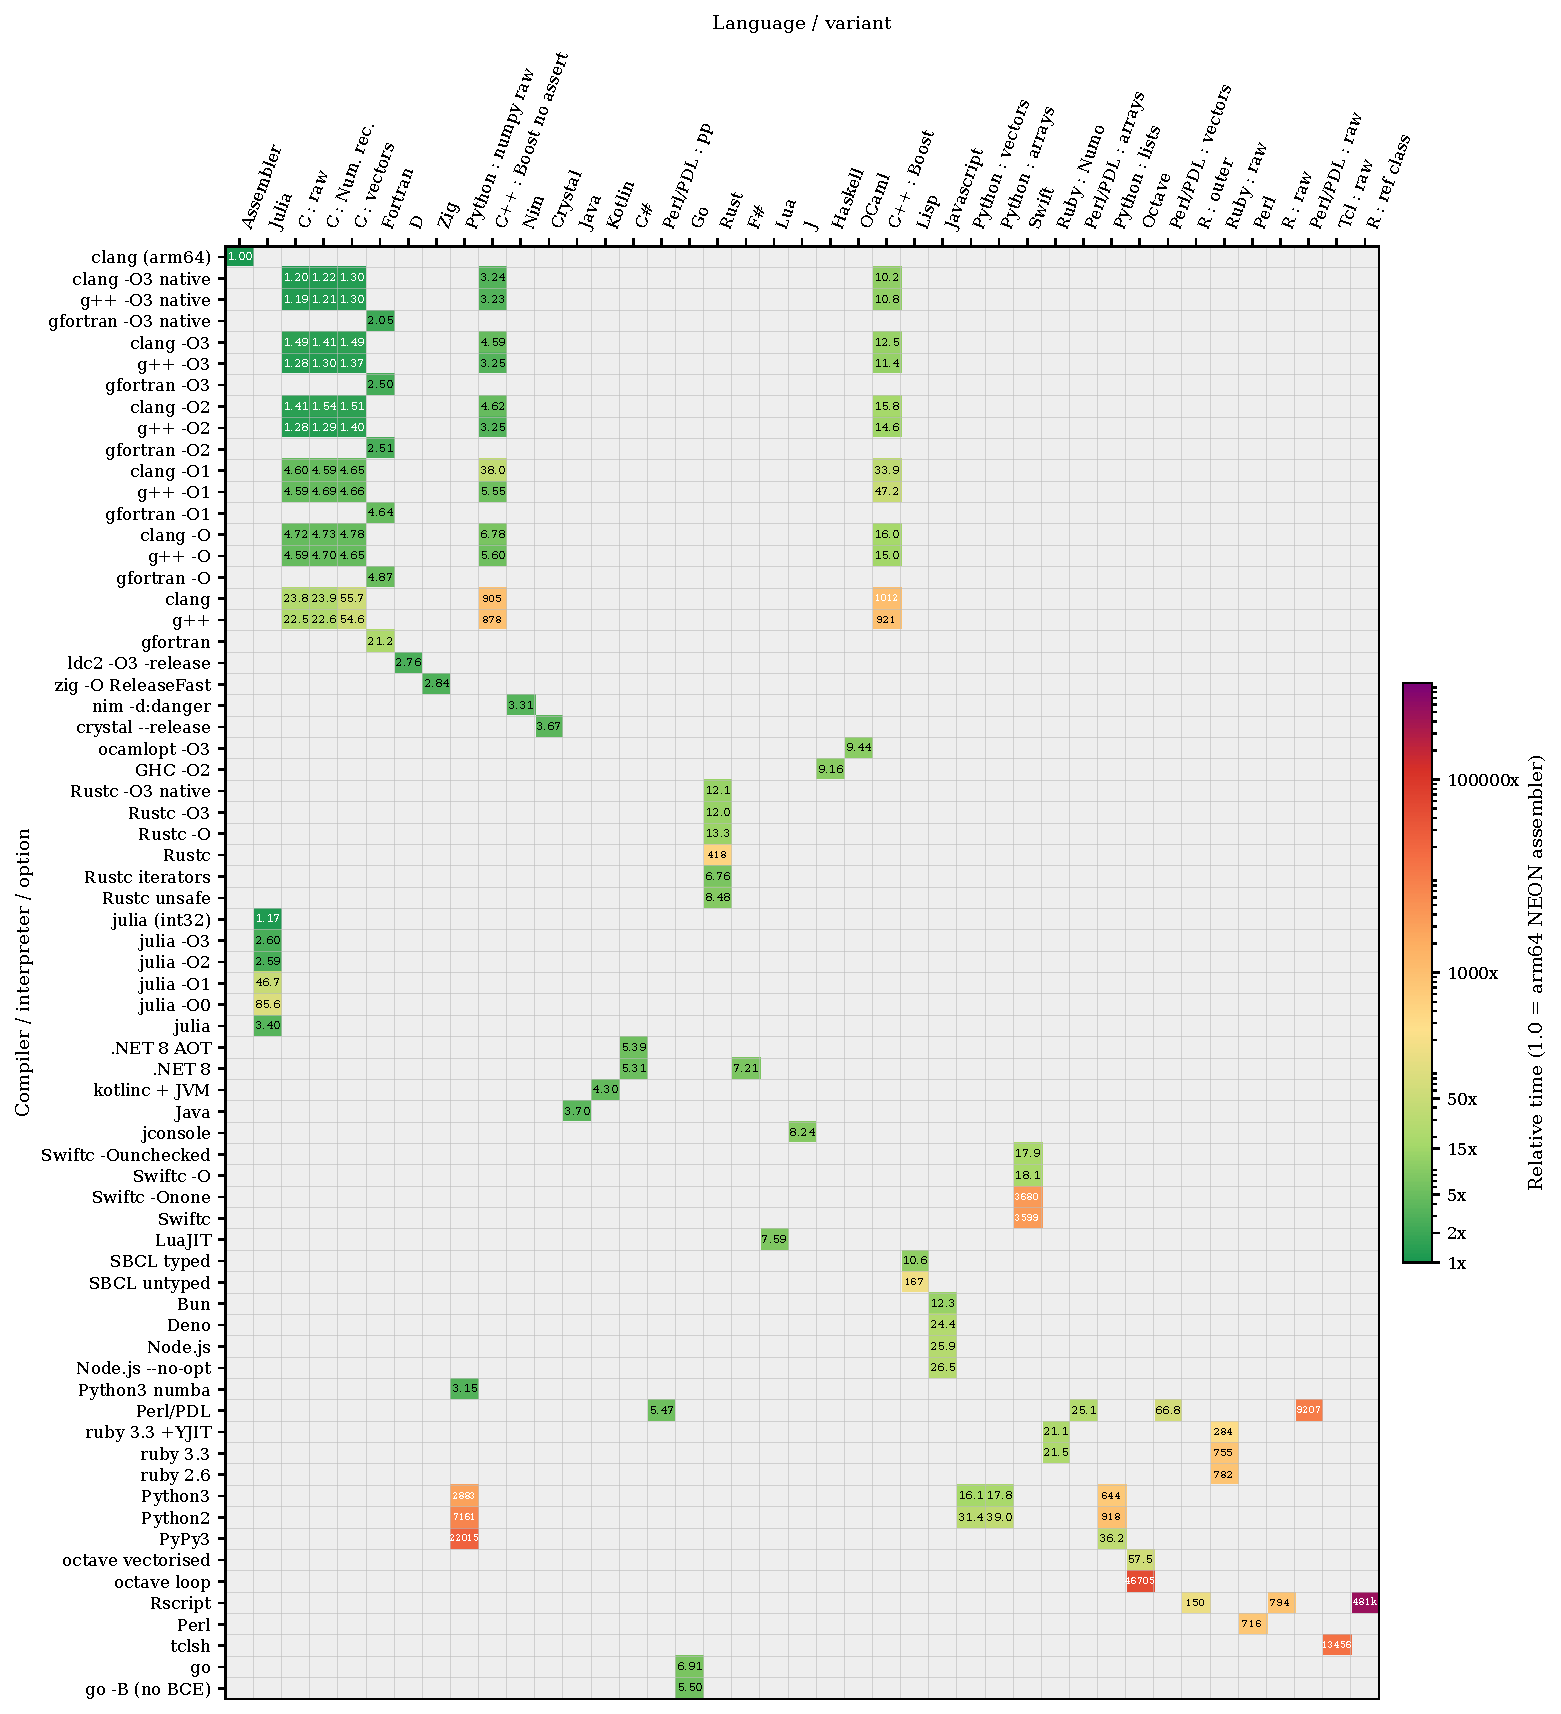
\includegraphics[width=\textwidth]{figs/fig1_heatmap.pdf}
\caption{The 2026 successor to Shortridge (2019) Figure~1. All 131
test variants on the same colour scale. Reference: hand-written
arm64 NEON assembler. Empty cells are language/compiler combinations
not run.}
\label{fig:heatmap}
\end{figure}

\noindent
The visual key:

\begin{center}\footnotesize
\begin{tabularx}{\textwidth}{clX}
\toprule
\textbf{Tier} & \textbf{Range} & \textbf{Examples} \\
\midrule
\swatch{tg1} 1 & 1.0\,--\,1.1 & arm64 assembler \\
\swatch{tg2} 2 & 1.1\,--\,2.5 & Julia int32, fastest C, Fortran \texttt{-O3 -march=native} \\
\swatch{tg3} 3 & 2.5\,--\,7   & Julia, D, Zig, Crystal, Nim, Java, C\#, Kotlin, Go, numba, Boost-no-assert, PDL::PP, Rust iter \\
\swatch{ty}  4 & 7\,--\,15    & F\#, LuaJIT, J, Haskell, OCaml, SBCL typed, Rust safe/unsafe, Boost-with-asserts \texttt{-O3}, Bun \\
\swatch{to1} 5 & 15\,--\,100  & numpy, Numo, PDL arrays/vectors, Octave vectorised, Swift \texttt{-O}, Node, Deno, unoptimised C/Fortran \\
\swatch{to2} 6 & 100\,--\,600 & R outer, SBCL untyped, Ruby +YJIT, Rust unoptimised \\
\swatch{tr}  7 & 600\,--\,15\,000 & \textbf{Python lists Py3}, Perl, Ruby raw, R raw, unoptimised Boost, Python lists Py2, Python numpy raw, Swift unoptimised, PDL raw, Tcl \\
\swatch{tp}  8 & $\geq 20\,000$ & PyPy + numpy, Octave loop, R ref-class \\
\bottomrule
\end{tabularx}
\end{center}

A per-language-family view of the same data, with min/max ranges
and geometric means across each family's variants, is shown in
Figure~\ref{fig:top30}. The distribution of all 131 results across
the eight tiers is shown in Figure~\ref{fig:tiers}, and a log-binned
histogram of the 131 individual values in
Figure~\ref{fig:hist}.

\begin{figure}[!htb]
\centering
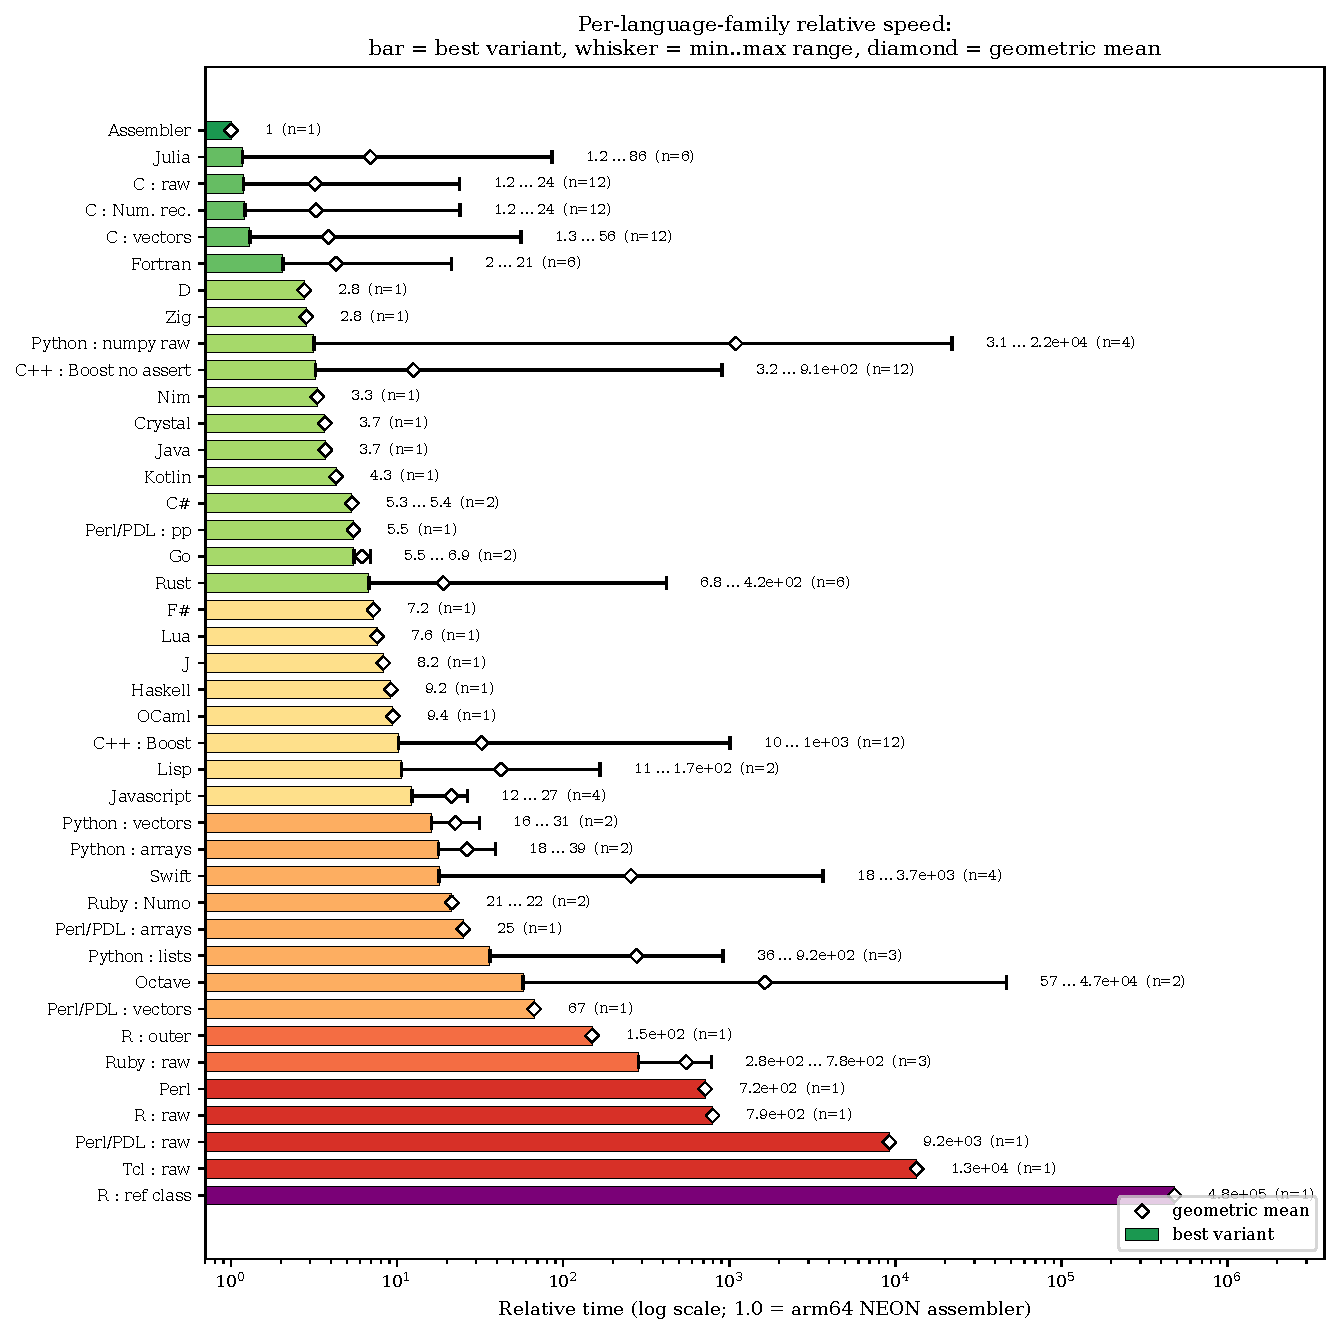
\includegraphics[width=0.95\textwidth]{figs/fig3_top30.pdf}
\caption{Per-language-family aggregate. The bar shows each family's
\emph{best} result; the whisker spans min..max across all variants
in that family; the diamond marks the geometric mean. Annotations
give the range and the number of variants ($n$). Multi-variant
families (C, Boost, Fortran, Julia, Rust, Python: numpy raw)
demonstrate how compiler/optimisation flags can move a single
language across two or more orders of magnitude --- but the
\emph{best} variant always determines the language's tier.}
\label{fig:top30}
\end{figure}

\begin{figure}[!htb]
\centering
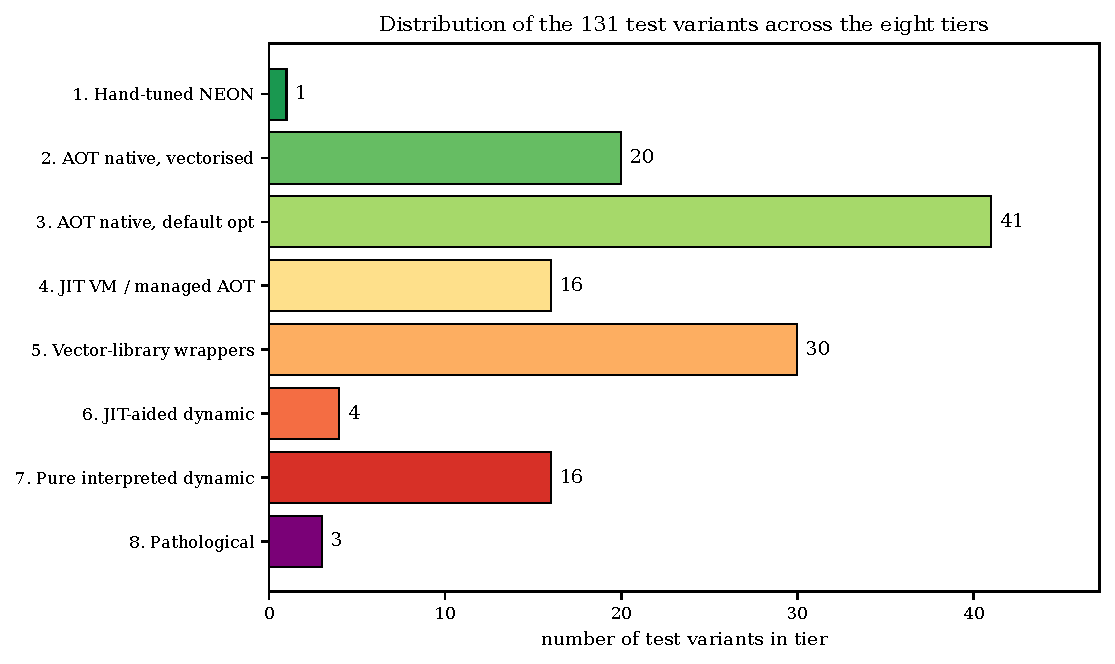
\includegraphics[width=0.85\textwidth]{figs/fig2_tiers.pdf}
\caption{Distribution of the 131 test variants across the eight
tiers (one bar per tier; counts annotated). The compiled-to-native
tiers (2 and 3) hold 47\% of all results; only one entry sits in
tier 1 (hand-tuned NEON), and three sit in tier 8 (pathological).}
\label{fig:tiers}
\end{figure}

\begin{figure}[!htb]
\centering
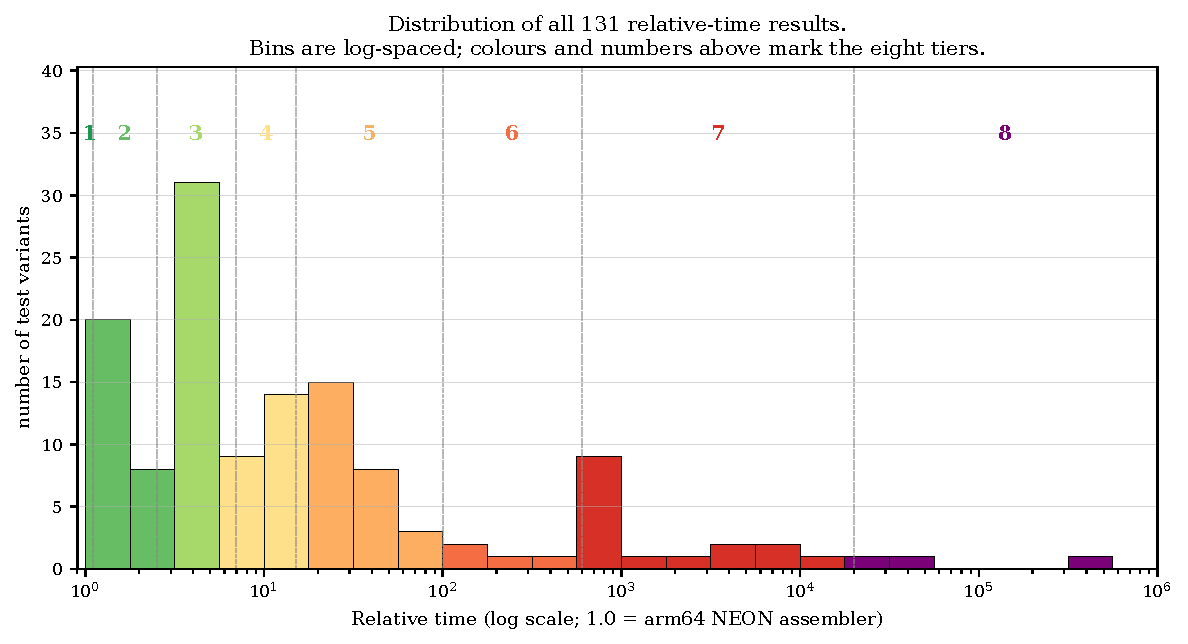
\includegraphics[width=0.95\textwidth]{figs/fig6_histogram.pdf}
\caption{Histogram of the 131 individual relative-time values on a
log scale. Bars are coloured by tier; tier numbers are repeated above
the histogram for reference. The bimodal shape is clear: a large
mass of compiled-to-native results in tiers 2--5 (relative speed
1--100$\times$), and a separate dynamic-interpreter cluster in tier
7 around $10^3\times$. The three pathological tier-8 outliers and the
single tier-1 hand-tuned assembler are visible at the extremes.}
\label{fig:hist}
\end{figure}

% ----------------------------------------------------------------------
\section{How the languages cluster}

The 131 results sort cleanly into the eight tiers shown above. Tier
boundaries are not arbitrary; each represents a concrete
architectural decision about how the language compiles or interprets
numeric loops.

\paragraph{Tier 1 --- hand-tuned NEON (1.00).}
Just the one entry: \texttt{cnrsub\_arm.s}, written by Shortridge in
2022 as a learning exercise. It beats the next-fastest result
(Julia int32 at 1.17$\times$) by about 17\%, and the fastest C
configuration (1.19$\times$) by about 19\%. This
is a transient state: M-series clang's auto-vectoriser will close the
gap in a release or two. In 2019 hand-written x86 assembler could
\emph{not} beat compilers, and that finding will return.

\paragraph{Tier 2 --- AOT to native, vector-instruction-using (1.1\,--\,2.5).}
Just C, C++, Fortran and Julia, when fully optimised with vector
instructions (\verb|-O2|/\verb|-O3| with \verb|-march=native| or
equivalent) --- plus Julia's int32 trick at the very top. Across
this whole tier, the optimised back-end produces almost identical
machine code; the language is doing little work the compiler cannot
undo. A 2019 finding that survives unchanged: most C/C++ approaches
produce essentially the same number once optimisation is turned on.
The other systems-tier languages split just below this. D, Zig,
Crystal and Nim land in tier 3, alongside the JIT-VM languages
(Java, C\#, Kotlin, Go). F\# at 7.21$\times$ has crossed just over
the tier-3/4 boundary into tier 4 (in 2019 it was tier 3). Optimised
Rust (in its iterator,
unsafe and \verb|-O3 native| forms), OCaml and SBCL-typed all sit
slightly lower in tier 4, because bounds checks, array layout or
type-information overhead leaves a small but visible cost on this
kernel. SBCL-untyped is a different case entirely and falls all
the way to tier 6.

\paragraph{Tier 3 --- compiled or JIT-compiled to native, no vector hints (2.5\,--\,7).}
Most of the dataset's compiled languages plus the JIT VMs land here:
D, Zig, Crystal, Nim, Java, C\# (JIT and AOT --- they coincide here),
Kotlin, Go, plus C/Fortran at \verb|-O|/\verb|-O1| and the various
Boost-no-assert configurations. This is the most populous tier of the
suite (41 entries). What unites it: the inner loop is compiled to
native code at some point, but without the vector-instruction hints
that move tier 2 ahead. D (2.76) and Zig (2.84) sit at the top, with
numba (3.15), Nim (3.31), Crystal (3.67) and Java (3.70) close
behind; Go default (6.91) is near the bottom. F\# at 7.21$\times$
has crossed just over the boundary into tier 4. Notably, \textbf{Perl/PDL::PP
(5.47) lives in this tier} despite being a Perl test --- because
its kernel is compiled C lowered through PDL::PP and called from
Perl as a single dispatch, the Perl-the-language wrapping costs are
amortised away (see \S\ref{sec:syntax} for the syntax detail).

\paragraph{Tier 4 --- harder cases of JIT and AOT (7\,--\,15).}
LuaJIT (7.59), J (8.24), Rust safe and unsafe at \verb|-O3 native|,
Haskell, OCaml, SBCL-typed, Bun, and the C++ Boost variants
\emph{with} assertions on. What unites this tier is the presence of
\emph{some} runtime check or abstraction the optimiser cannot fully
elide: Rust's bounds-check elision is incomplete in the indexed-loop
form; Boost's assertions add per-element checks; J's primitive
dispatch has unavoidable per-call overhead; OCaml's
\texttt{float array array} is row-pointer-indirect rather than
contiguous. All of these compile to native code, but none of them
reach the unconditional fast path of tier 3. (PDL::PP at 5.47 sits
just below this tier --- close enough that the boundary feels
slightly arbitrary; the tier 4 entries are paying $\sim\!2\!\times$
of optimal-C overhead from runtime checks, while PDL::PP is paying
$\sim\!1\!\times$ from its broadcasting macros.)

\paragraph{Tier 5 --- Vector-library wrappers (15\,--\,100).}
numpy ``vectors''/``arrays'', Ruby Numo, Perl/PDL arrays/vectors,
Octave vectorised. The kernels are compiled C; what is measured is
the per-element overhead of the vector library's broadcasting
machinery (PDL\_Indx arithmetic, slice descriptors, dtype dispatch,
the GIL on Python's side). Same floor everywhere --- the host
language is not the limiting factor.

\paragraph{Tier 6 --- JIT-aided dynamic (100\,--\,600).}
Just four entries: R outer (150), SBCL untyped (167), Ruby +YJIT
(284), and unoptimised Rust (418). A small mixed tier of
partially-compiled-but-not-fully or compiled-but-not-optimised
configurations. Ruby +YJIT is the prototypical entry: a method-level
JIT that gets ${\sim}\!2.7\!\times$ over plain Ruby but lacks the
analysis depth of LuaJIT or V8.

\paragraph{Tier 7 --- Pure interpreted dynamic (600\,--\,15\,000).}
Sixteen entries, of which the most representative are:
\textbf{Python lists CPython 3 (644)}, Perl (716), Ruby raw 3.3 (755),
R raw (794), unoptimised Boost C++ (878--1012), Python numpy raw Py3
(2\,883), Swift unoptimised ($\sim$3\,600), \textbf{PDL raw (9\,207,
after the 2026 \texttt{->at}/\texttt{->set} correction)}, and Tcl
(13\,456). Bytecode dispatch per operation, dynamic dispatch per
arithmetic op, no specialisation across types. The $\sim$20$\times$
spread within this tier reflects how heavy the per-bytecode-op work
is, not anything fundamental about the languages' type systems.
Bytecode dispatch per operation, dynamic dispatch per arithmetic op,
no specialisation across types. The 20$\times$ spread within this
tier reflects how heavy the per-bytecode-op work is, not anything
fundamental about the languages' type systems.

\paragraph{Tier 8 --- Pathological ($\geq 20\,000$).}
Octave loop, R ref-class, PyPy + numpy. Each of these
is a \emph{legitimate} coding choice that interacts catastrophically
with the language runtime's design. They are the most pedagogically
useful results in the suite --- if you understand \emph{why} each is
in this tier, you understand the language much better.

% ----------------------------------------------------------------------
\section{The vectorised-language picture}

Four language families (Python, Perl, Ruby, Octave) have one or
more ``vector-library'' idioms alongside their conventional one,
giving six rows of comparison in Table~\ref{tab:veclibs}. In each
case there is a dramatic difference.

\begin{table}[h]
\centering
\small
\begin{tabular}{lrrr}
\toprule
\textbf{Language} & \textbf{Loop tier} & \textbf{Vector tier} & \textbf{Speed-up} \\
\midrule
Python (numpy ``vectors'') & 644 (lists) & 16 & 40$\times$ \\
Python (numpy ``arrays'')  & 644 (lists) & 18 & 36$\times$ \\
Perl (PDL arrays)          & 716 (pure Perl) & 25 & 29$\times$ \\
Perl (PDL vectors)         & 716 (pure Perl) & 67 & 11$\times$ \\
Ruby (Numo)                & 755 (pure Ruby) & 22 & 35$\times$ \\
\textbf{Octave}            & \textbf{46\,705 (loop)} & \textbf{57 (vec)} & \textbf{813$\times$} \\
\bottomrule
\end{tabular}
\caption{Intra-language speed-ups from switching to the vectorised
idiom. Octave is in a class of its own.}
\label{tab:veclibs}
\end{table}

Octave's 813$\times$ spread between the loop and vectorised forms is
the dramatic centrepiece of the table (Figure~\ref{fig:octave}).
Both forms are \emph{idiomatic Octave}: a working scientist would
naturally write either one. Yet the loop form is among the slowest
results in the entire 131-test suite, while the vectorised form
sits in the same tier as numpy and Numo. (Perl/PDL has a smaller
but still wide same-language gap --- the per-element PDL ``raw''
form (9\,207$\times$, after the 2026 \texttt{->at}/\texttt{->set}
correction) versus the inline-C PDL::PP kernel (5.47$\times$) spans
about 1\,700$\times$ --- but the two forms there are not ``loop''
vs ``vectorised'' in the same idiomatic sense; PDL::PP is a
compiled C kernel embedded in a Perl script.)

\begin{figure}[!htb]
\centering
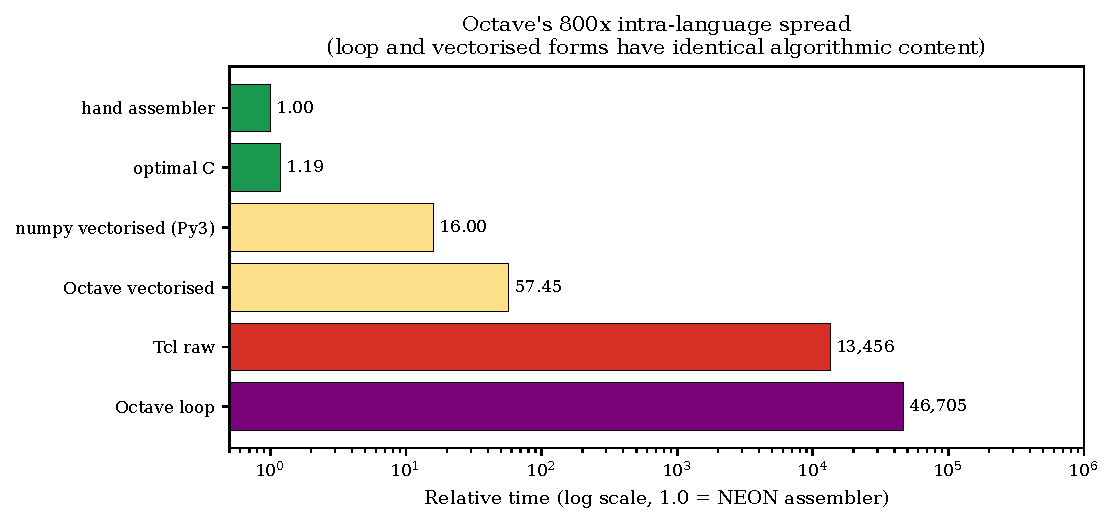
\includegraphics[width=0.85\textwidth]{figs/fig4_octave.pdf}
\caption{Octave's $\sim$810$\times$ intra-language spread. Both
implementations are idiomatic Octave; both compute the same answer.
The difference is whether the work is done by Octave's interpreter
(46\,705$\times$) or its compiled vector kernel (57$\times$).}
\label{fig:octave}
\end{figure}

A separate question is how the vector-library kernels compare to
each other. Once you cross into the compiled C extension, the host
language stops mattering:

\begin{center}\small
\begin{tabular}{lll}
\toprule
\textbf{Library} & \textbf{Host} & \textbf{Rel.~speed} \\
\midrule
PDL::PP (compiled C kernel) & Perl & \textbf{5.47} \\
numpy ``vectors''            & Python & 16.0 \\
numpy ``arrays''             & Python & 17.6 \\
Ruby Numo                    & Ruby & 21.5 \\
Perl/PDL arrays              & Perl & 25.1 \\
Octave vectorised            & Octave & 57.5 \\
Perl/PDL vectors             & Perl & 66.9 \\
\bottomrule
\end{tabular}
\end{center}

\noindent
The ordering is determined almost entirely by the cleverness of the
library, not the host language. PDL::PP sits ahead of every numpy
result, every Numo result, and every JavaScript engine. The
Perl-the-language overhead is not the limit; PDL's broadcasting
machinery is.

A particularly interesting case is the \textbf{J language} (tier 4,
8.24$\times$). J is a successor to APL: dynamically typed,
interpreted, with a heavily symbolic syntax --- yet it lands ahead of
Bun (12.29$\times$), Node.js (25.88$\times$), and Ruby Numo
(21.54$\times$, or 21.15$\times$ with YJIT). The whole benchmark is one expression:

\begin{lstlisting}
out =. y + (i. ny) +/ i. nx
\end{lstlisting}

\noindent
(``outer-product-add the row indices and column indices to make an
$iy+ix$ matrix, and add it to the input array $y$''). Because the
entire 20\,000-element kernel runs as one primitive call, J's
interpreter dispatch overhead is amortised away. J pays the same
``cross-into-compiled-C-once'' cost as numpy and Numo --- but its
broadcasting machinery is slimmer than the high-level array-library
wrappers, putting it ahead of every numpy/Numo/PDL-array result in
the suite. (J does not beat PDL::PP, which lands at 5.47$\times$:
PDL::PP is no longer wrapping at the array level but compiling a
small C kernel inline.)

The lesson, consistent with 2019's observation about numpy:
\emph{the vector-library tier is governed by the library, not the
language}. Choose your scientific stack on language ergonomics, and
trust that the underlying tensor library will produce roughly the
same number.

% ----------------------------------------------------------------------
\section{Notable syntaxes and language-specific optimisations}
\label{sec:syntax}

\paragraph{J --- array-orientation taken to the limit.}
The full J port is nine lines (most of which are argument parsing
and result-checking). The kernel itself is one expression:
\verb|y + (i. ny) +/ i. nx|, where \verb|i.| is range, \verb|+/|
is reduce-sum, and adjacent verbs compose. J's roots are in
Iverson's APL; the syntax is dense to the point of hostility but the
\emph{thinking} it encourages --- operate on whole arrays, never
write a loop --- is modern data science distilled. The performance
result (8.24$\times$) is largely a side-effect of this discipline:
when there are no loops, there is nothing for the interpreter to
slow down.

\paragraph{SBCL Common Lisp --- typed vs.\ untyped (15$\times$ difference).}
Two source files, identical except the typed variant adds:

\begin{lstlisting}[language=Lisp]
(deftype matrix () '(simple-array double-float (* *)))
(declaim (ftype (function (matrix fixnum fixnum matrix) (values))
                subr))
(defun subr (in-arr nx ny out-arr)
  (declare (type matrix in-arr out-arr) (type fixnum nx ny))
  ...)
\end{lstlisting}

\noindent
Untyped: 167.25$\times$ relative time (tier 6, alongside Ruby +YJIT
and R outer).
Typed: 10.63$\times$ (tier 4, alongside Haskell, OCaml and LuaJIT). This is
the most pedagogical single result in the dataset. SBCL is a
sophisticated whole-program compiler --- but it cannot know what
type a variable is unless told. With a few \verb|(declare (type ...))|
forms, generic arithmetic dispatch becomes inlined double-float
arithmetic and the inner loop becomes tight machine code. Without
them, every \verb|+| is a runtime polymorphic dispatch through SBCL's
generic-function tables.

A \textbf{16$\times$ speed-up for adding eight declarations to a
working program}. This is exactly the value proposition Julia
inherits from Lisp: write fully untyped code and it works; add types
to the hot loop and it gets fast.

\paragraph{PDL::PP --- compiled C inside a \texttt{.pl} script.}
PDL::PP compiles a small C kernel via \texttt{Inline::Pdlpp}. The
kernel itself is:

\begin{lstlisting}[language=Perl]
pp_def('csub',
   Pars => 'i(m,n);[o] o(m,n)',
   Code => '
      loop(n) %{
          loop(m) %{
            $o() = $i() + m+n;
          %}
      %}
   ');
\end{lstlisting}

\noindent
The Perl wrapping is essentially free --- once compiled, calling
\verb|$InArray->csub| dispatches into the compiled \texttt{.bundle}.
The 5.47$\times$ result is determined entirely by PDL's broadcasting
macros: \verb|loop()| expands to a PDL\_Indx-aware iterator with
slice-descriptor checks per element, not a flat C \verb|for|.

\paragraph{PDL ``raw'' --- a 2019 implementation choice corrected
in 2026.}
The original \texttt{csubpdl.pl} in Shortridge (2019) implemented
per-element access using \verb|$Output->slice($ix,$iy) .= ...|.
That choice was a mistake. \verb|->slice| constructs a one-element
\emph{slice piddle} on every read \emph{and} every write --- the
slice machinery is designed for sub-array views, not for scalar
access --- which dominates the per-element cost and produced an
artificially bad result of $\sim\!10^5\times$ relative time, by
far the worst Perl/PDL number in the 2019 figure. The
\emph{intended} primitive for scalar access in PDL is
\verb|->at($ix,$iy)| (read, returns a Perl scalar) and
\verb|->set($ix,$iy,$v)| (write, no slice piddle constructed).
This is the proper PDL analogue of numpy's \verb|ina[iy,ix]|
indexing and is what Shortridge meant the test to do.

This 2026 reprise replaces the 2019 form with the
\verb|->at|/\verb|->set| form. The corrected PDL raw result is
\textbf{9\,207$\times$}, about $11\times$ faster than the 2019
\verb|->slice| version, and now in the same broad ballpark as
Python numpy raw (2\,883$\times$, on CPython). It is still slow ---
you are still looping in Perl and crossing into C on every
element --- but it is no longer worst-of-suite. PDL raw now sits
in tier 7 alongside Tcl, R raw, Python lists Py2, and unoptimised
Boost; tier 8 (pathological) now contains just three entries ---
PyPy+numpy (22\,015), Octave loop (46\,705) and R reference-class
(481\,009). The
2019 paper's ``the per-element PDL access form is the second-worst
result in the suite'' is no longer true under this corrected
implementation.

The original \verb|->slice|-based test has been removed from the
benchmark suite; \texttt{csubpdl.pl} now contains the
\verb|->at|/\verb|->set| form. (The \texttt{csubpdl.pl} source
file in the repository carries an explanatory comment at the top
documenting the change.)

\paragraph{numba --- the Python decorator that JITs.}
\begin{lstlisting}[language=Python]
from numba import njit

@njit
def subr(In, Nx, Ny, Out):
    for iy in range(Ny):
        for ix in range(Nx):
            Out[iy, ix] = In[iy, ix] + ix + iy
\end{lstlisting}

\noindent
One decorator. \mbox{2\,883$\times$} $\rightarrow$ \mbox{3.15$\times$}: a
915$\times$ speed-up by adding a single decorator to a numpy-using
function. \textbf{Note that numba is not really doing anything
\emph{numpy}-specific here}: it is JIT-compiling a regular Python
loop, treating the numpy array as a typed contiguous double buffer.
It does not call into numpy's compiled C kernels at all. The
``numpy'' in the test name simply provides a strongly-typed
contiguous storage that numba's type-inference can specialise for;
the loop itself is then lowered to LLVM IR and from there to native
machine code that completely bypasses numpy's Python boundary. The
result is that numba performs essentially the same job that LuaJIT
or a Crystal compiler would perform on equivalent code: it turns
Python's per-element interpreter dispatch into a flat native loop.
This is the single most cost-effective speed improvement available
to a working scientist who has Python code in hand and a five-minute
time budget.

\paragraph{Crystal --- Ruby syntax with types.}
Identical-looking source code to Ruby, but Crystal infers types at
compile time and lowers to LLVM IR. Result: 3.67$\times$ ---
\emph{near C-class}. The same algorithm in Ruby (with YJIT) is
284$\times$; without YJIT, 755$\times$ (Ruby 3.3) or 782$\times$
(Ruby 2.6). Crystal demonstrates that
\textbf{the cost of being Ruby-the-language is not the syntax; it
is the dynamic dispatch}.

\paragraph{Kotlin = Java, F\# $\neq$ C\# (but close).}
Kotlin (4.30) lands slightly slower than Java (3.70) on the same
JVM. F\# (7.21) lands $\sim$36\% slower than C\# (5.31) on the same
.NET runtime. Both are explainable: Kotlin's nullability-checked
types compile to a few additional method calls the JIT can inline
\emph{almost-but-not-quite} away; F\#'s discriminated unions and
option types add small constants to imperative loops. \textbf{Within
runtime-pairs, the source language matters at the
20--40\% level, the runtime matters at the order-of-magnitude
level.}

\paragraph{LuaJIT and J --- the frontier of ``dynamic but fast''.}
LuaJIT (7.59) and J (8.24) are the two cleanest demonstrations that
a dynamically-typed language can run at AOT-compiled speeds. They
get there by entirely different means:

\begin{itemize}
\item \textbf{LuaJIT} is a \emph{tracing JIT}: it observes hot loops,
infers type-specialised machine code for them, and emits inline
assembly. The user writes ordinary Lua; the JIT does everything.

\item \textbf{J} is \emph{not} JIT-compiled at all --- it is
interpreted, but its primitive operations are themselves tight C
kernels and the \emph{language} discourages writing per-element
loops. The user gets speed by accepting the array-oriented idiom.
\end{itemize}

\noindent
These are the two primary paths to closing the dynamic-language
performance gap. PyPy (Python's tracing JIT) takes the LuaJIT path
but lands further behind, because Python's dynamic semantics are
considerably more complex than Lua's, leaving the JIT less to work
with.

% ----------------------------------------------------------------------
\section{Anomalies}

The benchmark surfaced six results that were not predictable from
first principles, all of which are pedagogically valuable.

\paragraph{PyPy + numpy is 600$\times$ \emph{slower} than PyPy + Python lists.}

\begin{center}\small
\begin{tabular}{lr}
\toprule
\textbf{Configuration} & \textbf{Rel.~speed} \\
\midrule
PyPy + Python lists (\texttt{csubraw.py}) & 36 \\
CPython + numpy raw (\texttt{csubnp.py}) & 2\,883 \\
\textbf{PyPy + numpy raw (\texttt{csubnp.py})} & \textbf{22\,015} \\
\bottomrule
\end{tabular}
\end{center}

\noindent
This is the single largest counter-intuitive finding in the new
data. Almost every Python programmer has heard ``PyPy is faster
than CPython''; almost none know that this is \emph{false} for
numpy-heavy code, sometimes by an order of magnitude. The
mechanism: PyPy implements its own internal object model, designed
for the tracing JIT to reason about. To support compiled extensions
like numpy that target the CPython C API, PyPy provides a shim
called \texttt{cpyext} that translates between PyPy objects and the
shapes numpy expects. Every call into a numpy C extension crosses
\texttt{cpyext}, which is much slower than CPython's native fast
path. For tight loops that invoke numpy thousands of times, the
per-call \texttt{cpyext} cost dominates. The JIT cannot help because
the JIT cannot trace into compiled C.

Working scientists' takeaway: \textbf{PyPy is only beneficial for
\emph{pure} Python code}. As soon as you cross into a
numpy/scipy/scikit C extension, it becomes a net slowdown. CPython
remains the right choice for the numpy-using majority of scientific
Python.

\paragraph{Octave loop --- worst-of-suite performance from idiomatic code.}
Octave's element-wise loop runs at 46\,705$\times$ relative time ---
slower than Tcl, slower than R-raw, slower than PyPy+numpy
(22\,015$\times$), only beaten in the bottom of the suite by R
ref-class (481\,009$\times$). Yet the source is \emph{idiomatic};
see Figure~\ref{fig:octave}. The hot kernel of \texttt{csubraw.m} is
the obvious nested-loop translation:

\begin{lstlisting}
for iy = 0:ny-1
   for ix = 0:nx-1
      out(iy+1, ix+1) = ina(iy+1, ix+1) + ix + iy;
   end
end
\end{lstlisting}

\noindent
The vectorised form (\texttt{csubvec.m}) does the same thing in one
broadcast. Outside the timed loop, two short index vectors are built
once --- a 1$\times$$N_x$ row and an $N_y$$\times$1 column:

\begin{lstlisting}
ix_row = 0:nx-1;       % 1 x nx (row vector)
iy_col = (0:ny-1)';    % ny x 1 (column vector, transposed)
\end{lstlisting}

\noindent
The hot kernel is then a single expression. Octave broadcasts the
row across all rows of \texttt{in}, the column across all columns,
and adds:

\begin{lstlisting}
out = in + ix_row + iy_col;
\end{lstlisting}

\noindent
That single expression runs 813$\times$ faster (57$\times$ relative
time) than the nested loop above. \textbf{Octave is a domain-specific
language for vectorised arithmetic}; the scalar interpreter exists
because it must, not because it should be used. Modern Matlab
(R2015b+) ships a JIT that specifically targets this anti-pattern ---
Octave does not.

\paragraph{Perl/PDL raw and Python numpy raw --- traps disguised as
idiomatic code.}
Perl/PDL raw lands at 9\,207$\times$ (after the 2026
\verb|->at|/\verb|->set| correction), and Python numpy raw at
2\,883$\times$ --- markedly worse than their \emph{plain}
pure-language counterparts (Perl raw 716$\times$, Python lists
644$\times$). The Perl factor is the more dramatic of the two: PDL
raw is $\sim\!13\!\times$ worse than pure Perl, while CPython numpy
raw is $\sim\!4.5\!\times$ worse than CPython lists. Both are surprising results until one notices
what ``raw'' actually means in those tests: \textbf{a host-language
loop that calls into the C array library on every single element}.
For PDL, each iteration calls \verb|$ina->at($ix,$iy)|, which
crosses the Perl-to-C boundary, dereferences the piddle's storage,
and returns a Perl scalar --- and then \verb|$out->set($ix,$iy,$v)|
does the inverse on the write side. For numpy, each
\verb|ina[iy,ix]| traverses numpy's \verb|__getitem__| machinery,
builds a Python scalar from the underlying C buffer, and returns it
through the C-API; the assignment side does the inverse. The
host-language interpreter overhead is then \emph{added} to that,
not amortised away. Both ``raw'' tests are slower than the
equivalent code written using only the host language's native data
structures, because they pay the host's per-iteration cost
\emph{plus} the C-extension's per-call cost.
The ``raw'' label is misleading: these are not vectorised operations
in the J/PDL-arrays/numpy-arrays sense (one C-side broadcast); they
are scalar accesses into a vectorised data structure, which is the
worst of both worlds. The only thing the user is saving by using
PDL/numpy in this style is the in-memory layout (a contiguous C
buffer) --- and on this benchmark, that saving is not enough to pay
for the per-element traversal overhead.

\paragraph{R reference class --- 481\,009$\times$ (the 2019 outlier).}
Inherited from the 2019 study with the same root cause. R's
reference classes are closure-based; modifying a single field copies
the entire encapsulated state. For an array-modifying method called
per-element, this means an $N\times N$ copy per element write ---
quadratic-times-iterations work for what should have been
constant-per-call work. The 2019 paper reported about 1.5\,M$\times$
on x86; the 2026 number is about 481\,000$\times$ on arm64 (a faster
assembler baseline divides into a different relative number). The lesson
is unchanged: \emph{idiomatic code can collide catastrophically with
a language's runtime model.}

\paragraph{OCaml --- \texttt{Bigarray.Array2} slowdown vs.\ \texttt{float array array}.}
OCaml is widely advertised as ``within 2--3$\times$ of C''. The
first version of the OCaml port used \texttt{Bigarray.Array2}
(intended specifically for numerical work) and ran at $\sim$120$\times$
optimal C --- a catastrophic gap. Switching to OCaml's native
\texttt{float array array} (unboxed per-row arrays of doubles) cut
the time by $\sim$13$\times$, landing at 9.44$\times$. The mechanism is
per-row allocation overhead: \verb|Array2.slice_left| allocates a
fresh \verb|Array1| view per call, defeating tight-loop optimisation.
Direct 2D access via \verb|arr.{iy, ix}| is no faster because
\verb|Bigarray|'s index-conversion macro is heavier than hand-rolled
multiplication. The lesson: even within ``fast OCaml,'' data-layout
choice produces order-of-magnitude differences. The documented
``near-C'' performance in the OCaml literature assumes
\texttt{float array} not \texttt{Bigarray}.

\paragraph{Julia int32 --- 1.17$\times$ through one type-coercion change.}
The original Julia test (using floats throughout) ran at about
3.40$\times$. Changing one expression to use int32 arithmetic for
the indices --- a hint Shortridge added in 2019 in response to
ADASS feedback --- produces 1.17$\times$. \textbf{A two-line code
change reaching the second-fastest result in the entire suite,
beaten only by hand-written assembler.} This result most strongly
supports the 2019 paper's recommendation of Julia for new scientific
work.

\paragraph{D and Zig --- modern systems languages, identical performance.}
D's LDC compiler and Zig's stage 0 backend are both LLVM-based, both
producing machine code that lands within $\sim$3\% of each other
(D 2.76$\times$, Zig 2.84$\times$) --- within the measurement noise
of the same number. Two languages with
very different design philosophies (D: optional GC, ranges,
template-heavy; Zig: manual memory, comptime, no hidden control
flow) compile to essentially the same SSA-IR shape on this benchmark
after the LLVM optimiser runs. The implication: \textbf{LLVM-IR-emitting
languages are converging at the back-end}. Differences in front-end
design rarely survive \verb|-O3|.

\paragraph{Swift --- a $\sim\!200\!\times$ optimisation cliff.}
Swift's relative numbers are striking: \verb|swiftc| (default, which
is \verb|-Onone|) lands at 3\,599$\times$, \verb|-Onone| explicit at
3\,680$\times$, but \verb|-O| brings this down to 18.14$\times$ and
\verb|-Ounchecked| to 17.91$\times$. That is a $\sim\!200\!\times$
swing from one optimisation flag --- one of the largest
\verb|-O0|/\verb|-O| gaps of any language in the suite, comparable
to C++ Boost-no-assert (which goes from $\sim\!900\!\times$ at
\verb|-O0| to $\sim\!3\!\times$ at \verb|-O3 native|, a ratio of
$\sim\!280\!\times$). The reason is structural:
Swift's runtime carries several costs that are normally invisible
because the optimiser eliminates them, but which dominate when it does
not. An idiomatic \verb|Array<Array<Float>>| element access at
\verb|-Onone| pays:
\begin{itemize}
\item \textbf{ARC retain/release} on the inner row reference each
time the subscript is taken (Swift's automatic reference counting is
a runtime call, not free);
\item \textbf{Generic dispatch} through the \texttt{Collection}
protocol witness table on every \texttt{subscript(\_:)} call ---
Swift's generics are not specialised at \verb|-Onone|;
\item \textbf{Bounds checking} on each access;
\item \textbf{Copy-on-write checks} on the array storage.
\end{itemize}
At \verb|-O|, the optimiser specialises \verb|Array<Float>.subscript|
for the concrete type, devirtualises the Collection-protocol calls,
hoists ARC operations out of the loop or elides them entirely, and
inlines the inner loop down to plain pointer arithmetic. The 200$\times$
spread is the cost of those four runtime mechanisms, end-to-end, with
no compiler help. Shortridge (2019) saw essentially the same
$\sim\!470\!\times$ behaviour on the original x86 hardware --- this
is a property of the language's runtime model, not the platform. The
practical takeaway: \emph{never benchmark Swift code without
\textnormal{\texttt{-O}}}; the result will mislead you by two orders
of magnitude.

% ----------------------------------------------------------------------
\section{Comparison with 2019}

A handful of languages were in both studies. Where comparable, the
relative-speed ordering is preserved, but several quantitative numbers
have shifted. Figure~\ref{fig:compare} shows the comparison
graphically.

\begin{figure}[!htb]
\centering
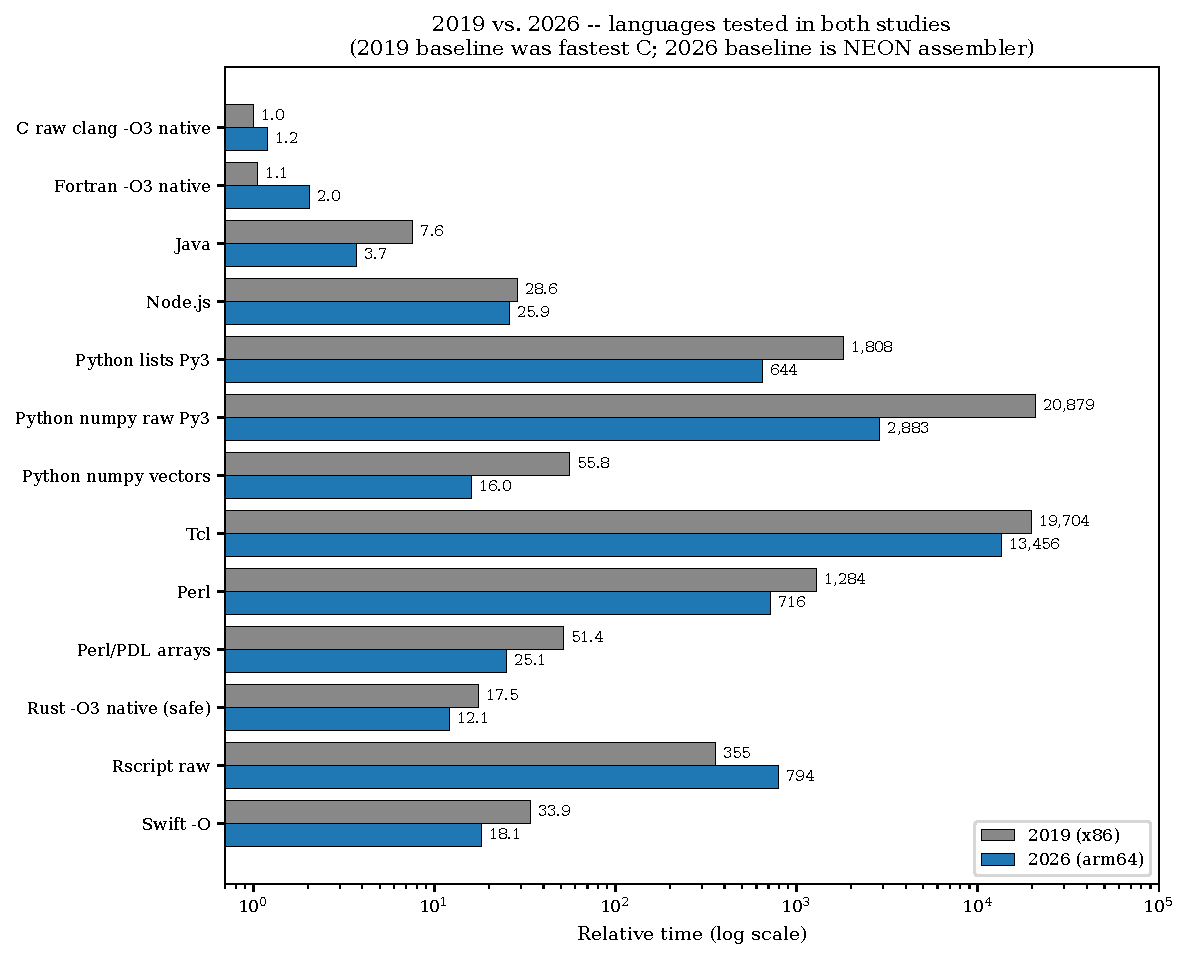
\includegraphics[width=0.95\textwidth]{figs/fig5_2019_vs_2026.pdf}
\caption{The 13 results that have a direct counterpart in both
studies (Shortridge 2019, x86; this 2026 reprise, arm64). The 2019
baseline was the fastest C; the
2026 baseline is hand-written NEON assembler. Most languages stayed
in their tier or improved; the qualitative ordering is unchanged.}
\label{fig:compare}
\end{figure}

\noindent
The qualitative picture is unchanged. Language-tier ordering is
robust across hardware platforms and seven years of compiler
evolution. \textbf{Where languages have improved, they have done so
within their tier}, not by jumping to a higher one. The exception is
Python, where numpy's fast path has gotten substantially faster, and
(more importantly) numba has emerged as a near-C JIT for numpy code.

% ----------------------------------------------------------------------
\section{Recommendations by use case}

The 2019 paper closed with the modest recommendation to ``look
closely at the performance you are getting'' and to consider Julia or
Rust for new scientific work. Seven years on, the dataset supports
more specific advice.

\paragraph{Writing the inner loop of an astronomical pipeline.}
Use \textbf{C, Fortran, or Julia} with full optimisation
(\verb|-O3 -march=native|). All three sit in tier 2 (1.1\,--\,2.5$\times$).
The choice between them is ergonomic, not performance-driven. C if
you need to interface with FITS libraries or call from Python;
Fortran if your group is already invested; Julia if you want an
interactive REPL and modern syntax with the same back-end performance.

If you need every last percent of speed and have NEON-shaped data,
hand-written arm64 assembly is currently 17--19\% faster than the best
compilers. This will not last. It is also not a recommendation for
production code.

\paragraph{Writing tools / utilities / glue around scientific libraries.}
Use \textbf{Python with numpy} (or PDL if you are already in Perl).
Once your hot loop is in a vector-library call, the host language
matters very little (tier 5, 15\,--\,100$\times$). For the small
fraction of work where Python's per-element path is hit anyway, add
\verb|@njit| from numba --- nearly $10^{3}\,\times$ speed-up for one decorator,
no recompilation, no rewriting.

Do \textbf{not} use PyPy if your code calls into numpy. PyPy is a
substantial \emph{slowdown} for numpy-heavy work (tier 8). PyPy is
only appropriate if your hot loop is genuinely pure-Python.

\paragraph{Prototyping in an interactive scientific REPL.}
\textbf{Julia} (1.1\,--\,3$\times$) is the best choice the dataset
offers. It has the responsiveness of Python, the performance of C,
and a single syntax across all tiers (no need to learn numpy idioms
or write a C extension). The 2019 paper's enthusiasm has been
validated.

For groups already invested in Python, the
\verb|numpy + numba + matplotlib| stack remains pragmatic.

\paragraph{Idiomatic OO code with serious performance.}
\textbf{C\# / .NET} (5.31$\times$, JIT) or \textbf{Java / OpenJDK}
(3.70$\times$) are both strong choices. F\# (7.21) and Kotlin (4.30)
sit just behind their C-family siblings on the same runtimes ---
choose for syntax, not speed. If your performance budget extends a
bit further, \textbf{Crystal} (3.67) or \textbf{Go} (5.5\,--\,6.9) are
AOT-compiled alternatives.

\paragraph{Modern systems language with memory safety.}
\textbf{Rust} (6.8\,--\,13.3, depending on idiom) is the obvious
choice and has the strongest ecosystem of the new systems languages.
\textbf{D} (2.76) and \textbf{Zig} (2.84) are both \emph{faster}
than safe Rust on this benchmark, and demonstrate that a memory-safe
language can still land at C speed when the design lets the
optimiser see through the abstractions. Rust is the right answer for
most groups in 2026; Zig and D are right answers for specific
projects.

\paragraph{Teaching what ``high performance'' looks like.}
Run your students this benchmark on three Octave configurations: the
loop variant, the vectorised variant, and the same algorithm in C.
The 813$\times$ spread between Octave's two idioms is the most vivid
single-language demonstration of ``use the language fast path'' in
any language we tested. Then run it again in SBCL with and without
type declarations. The 16$\times$ spread there shows the same lesson,
applied to type information.

\paragraph{Demonstrating that language design matters.}
Compare these four results from the dataset:

\begin{center}\small
\begin{tabular}{lr}
\toprule
Python lists, CPython     & 644 \\
Python lists, PyPy        & 36 \\
Python lists with \verb|@njit| numba & $\approx$ 3 \\
Hand-written C            & 1.19 \\
\bottomrule
\end{tabular}
\end{center}

\noindent
\textbf{Nearly three orders of magnitude} (644 to 1.19 spans a
factor of $\sim$540) for what a working scientist can plausibly
think of as ``the same problem'' in Python, depending on which
runtime processes the source. The first three rows are even
\emph{the same source file}: switching from CPython to PyPy is
zero code change; adding a numba decorator is one line and
requires switching from a list to a numpy array. The C version
requires a rewrite. This is the broadest single point about ``how
fast can a language go'' the benchmark can demonstrate.

\paragraph{Combinations to avoid.}
A few combinations the dataset shows are genuinely poor choices for
inner-loop scientific work, and which are not just slow but which
\emph{surprise} their users with how slow they are:

\begin{itemize}
\item Octave element-wise loops (46\,705$\times$). Vectorise instead.
\item R reference classes for in-place array updates (481\,009$\times$).
\item Per-element PDL access (9\,207$\times$, after the 2026 \texttt{->at}/\texttt{->set} correction). Use PDL's vectorised forms.
\item numpy raw element-wise loops on PyPy (22\,015$\times$). Use CPython.
\end{itemize}

\noindent
These are pathological \emph{not} because they cannot be made faster
but because their idiomatic surface form looks like normal code.

% ----------------------------------------------------------------------
\section{Closing thoughts}

The 2019 paper's headline --- \emph{this code is over 1\,000\,000
times faster than that code} --- was true then. In this 2026 run
the corresponding fastest-to-slowest spread is about
481\,000$\times$: smaller than the 2019 headline, but still
pedagogically the same result. The seven-year gap has widened the
variety of points along that range.

What the new languages reveal is more nuanced. The compiled-systems
tier has converged: Crystal, D, Zig, Nim, Go, OCaml, SBCL-typed,
optimised Rust idioms, and Haskell all sit in a tight band between
2.8 and about 13. Different
front-ends, different paradigms (lazy, OO, functional, imperative),
but the same LLVM-class back-ends produce the same shape of machine
code. Front-end ergonomics now drive the choice, not measured
performance.

The dynamic-language tier has bifurcated. CPython, plain Ruby, plain
R, Perl, and Tcl remain in the 600\,--\,15\,000$\times$ range --- slow
but at least predictable. Above them, a new ``JIT-aided dynamic''
zone now spans tiers 4--6: at tier 4, LuaJIT (7.59) and Bun (12.29);
at tier 5, PyPy lists (36) and the V8-based JavaScript engines Node
(26) and Deno (24); at tier 6, Ruby +YJIT (284) and R outer (150).
The most populous tier in the 2026 dataset is tier 3 (41 entries) ---
the tight band of ``compiled or JIT-compiled to native, no vector
hints'' results into which essentially all of D, Zig, Crystal, Nim,
Java, C\#, Kotlin, Go, plus C/C++/Fortran at \verb|-O|/\verb|-O1|,
now fall. JIT compilation has gone mainstream, and most languages
now have \emph{some} path to it.

The vector-library tier (numpy, PDL, Numo, Octave) is unchanged in
character but has more entrants. It remains the single
highest-value option for scientific Python users --- and PDL::PP, in
particular, is the highest-leverage way to write a hot kernel inside
a \texttt{.pl} script.

And, finally, the most pedagogically rich finding of the whole
exercise: \textbf{language and runtime are separable}. The same
language can move by factors of several to nearly three orders of
magnitude depending on which runtime, compiler, type information or
fast path is used: Ruby raw at 755$\times$ vs.~Ruby +YJIT at
284$\times$ (a factor of $\sim$2.7); SBCL untyped at 167$\times$
vs.~SBCL typed at 11$\times$ ($\sim$16$\times$); CPython lists at
644$\times$ vs.~PyPy lists at 36$\times$ ($\sim$18$\times$); and
CPython numpy raw at 2\,883$\times$ vs.~numba at 3.15$\times$ ($\sim$
915$\times$, the largest such factor in the Python family). Even
this is exceeded by the Perl family: PDL raw vs.~PDL::PP, after the
2026 \texttt{->at}/\texttt{->set} correction to the raw form, is
9\,207$\times$ vs.~5.47$\times$ = $\sim$1\,683$\times$, the largest
single-language fast-path factor in the dataset. The benchmark makes explicit what
scientific programmers often do implicitly when they reach for
\texttt{numpy}, PDL::PP, numba, type declarations or a JIT runtime.

\bigskip
\noindent
\textit{The original paper's appendix on R reference classes ---
``a cautionary tale, some attempts to optimise can backfire'' ---
remains the appropriate cautionary tale.}

% ----------------------------------------------------------------------
\section*{References}
\addcontentsline{toc}{section}{References}

\begin{itemize}\small
\item Shortridge, K. 2019. ``Compilers, languages, options, and
astronomical images.'' \emph{Astronomical Data Analysis Software and
Systems XXIX}, ASP Conference Series, Paper P9-17.\\[2pt]
Conference paper PDF (4 pages):
\url{https://github.com/KnaveAndVarlet/ADASS2019/blob/master/P9-17.pdf}\\
Poster:
\url{https://github.com/KnaveAndVarlet/ADASS2019/blob/master/LanguagesAndImageProcessing.pdf}\\
Full write-up (53 pages, the per-language deep dive):
\url{https://github.com/KnaveAndVarlet/ADASS2019/blob/master/FullWriteUp.pdf}
\item Shortridge, K. 2019. \texttt{KnaveAndVarlet/ADASS2019}
(GitHub repository). All source code for the benchmark, including
the original 2019 language ports, the test harness \texttt{Run.py},
and the colour-coded results figure used as Figure~1 of the
conference paper.\\
\url{https://github.com/KnaveAndVarlet/ADASS2019}
\item Shortridge, K. 2022. \texttt{cnrsub\_arm.s}. Hand-written
arm64 NEON port of the benchmark kernel, contributed to the
repository in 2022 as a follow-up to the 2019 study. Used as the
1.00$\times$ reference in this 2026 reprise.
\item Glazebrook, K. \& Soeller, C. 1996--present.
\textbf{PDL --- The Perl Data Language.} First publicly released as
PDL 1.00 in October 1996. Project home page:
\url{https://pdl.perl.org/}. ``Day 24: Perl Data Language
reflections,'' PDL Advent Calendar 2024:
\url{https://pdl.perl.org/advent/blog/2024/12/24/reflections/}.
For background on the language and its origins, see
\emph{Perl Data Language} on Wikipedia
(\url{https://en.wikipedia.org/wiki/Perl_Data_Language}).
\item Numo (Ruby's numerical array library) --- the Ruby analogue
of numpy, used for the ``Ruby : Numo'' tests:
\url{https://github.com/ruby-numo/numo-narray}.
\end{itemize}

% ----------------------------------------------------------------------
\appendix
\section{Files}

The complete updated benchmark suite lives in
\texttt{ADASS2019/} (alongside \texttt{tools/}, \texttt{logs/} and
\texttt{reports/} as siblings of that directory):

\begin{itemize}\small
\item \texttt{Run.py} --- the harness, with bootstrap for
\texttt{tools/}-installed toolchains and conda environments.
\item \texttt{cnrsub\_arm.s} --- Shortridge's hand-written arm64 NEON
port (the reference implementation).
\item Source files: \texttt{csubraw.cs}, \texttt{csubraw.fs},
\texttt{csubraw.go}, \texttt{csubraw.zig}, \texttt{csubraw.d},
\texttt{csubraw.nim}, \texttt{csubraw.lua}, \texttt{csubraw.kt},
\texttt{csubraw.rb}, \texttt{csubraw.ml}, \texttt{csubraw.lisp},
\texttt{csubraw-typed.lisp}, \texttt{csubraw.hs}, \texttt{csubraw.cr},
\texttt{csubraw.m}, \texttt{csubvec.m}, \texttt{csubpdlpp.pl},
\texttt{csubnumo.rb}.
\item \texttt{run22.log} --- the canonical reference run (this
report's source numbers).
\item \texttt{tools/} --- local installs (Julia, Rust, Bun, Deno,
Go, LuaJIT, .NET 8, Crystal, J, PyPy, Zig, LDC, Nim, GHC,
custom YJIT-built Ruby, Boost headers).
\item Conda envs: \texttt{adass-r}, \texttt{adass-py2},
\texttt{adass-rb}, \texttt{adass-sbcl}, \texttt{adass-ocaml},
\texttt{adass-kotlin}.
\item \texttt{make\_figures.py} --- reproduces the five figures in
this report from \texttt{run22.log}.
\end{itemize}

\section{Reproducibility}

The benchmark and report assume the four-directory layout described
in Appendix~A. From a working copy of that layout:

\begin{lstlisting}[language=bash]
# Run the benchmark (~6 minutes wall clock):
cd ADASS2019 && python3 Run.py | tee ../logs/runN.log

# Update the frozen reference and regenerate figures:
cp ../logs/runN.log ../reports/run22.log
cd ../reports && python3 make_figures.py

# Recompile this document:
pdflatex Report-2026.tex && pdflatex Report-2026.tex
\end{lstlisting}

\noindent
Output sorted by relative speed appears at the bottom of the run,
after the per-test \texttt{Rept: ... Elap: ... 1K Iter:} lines and
the \texttt{Fastest combination is ...} marker.

% ----------------------------------------------------------------------
\section{Raw relative-time outputs}
\label{app:raw}

The complete sorted list of all 131 test variants from
\texttt{run22.log} follows. The \textbf{Tier} column carries the
same colour-coding as Figure~\ref{fig:heatmap} (green = fastest,
purple = pathological); \textbf{Rel.\ time} is the geometric ratio
to the hand-tuned arm64 NEON assembler (1.00); \textbf{ms / 1k iter}
is the absolute time per 1000 iterations of the kernel, in
milliseconds. This appendix is auto-generated from the canonical
log by \texttt{make\_raw\_table.py}; running that script after
replacing \texttt{run22.log} with a newer benchmark output will
regenerate the table verbatim.

\begingroup
\footnotesize
\setlength{\tabcolsep}{4pt}
\begin{longtable}{@{}clllr@{}}
\toprule
\textbf{Tier} & \textbf{Rel.\ time} & \textbf{Family} & \textbf{Variant} & \textbf{ms / 1k iter} \\
\midrule
\endfirsthead
\multicolumn{5}{l}{\emph{(continued from previous page)}} \\
\toprule
\textbf{Tier} & \textbf{Rel.\ time} & \textbf{Family} & \textbf{Variant} & \textbf{ms / 1k iter} \\
\midrule
\endhead
\midrule
\multicolumn{5}{r}{\emph{continued on next page}} \\
\endfoot
\bottomrule
\endlastfoot
\swatch{tg1} & 1.00 & Assembler & clang (arm64) & 0.0011 \\
\swatch{tg2} & 1.17 & Julia & julia (int32) & 0.0013 \\
\swatch{tg2} & 1.19 & C : raw & g++ -O3 native & 0.0013 \\
\swatch{tg2} & 1.20 & C : raw & clang -O3 native & 0.0013 \\
\swatch{tg2} & 1.21 & C : Num. rec. & g++ -O3 native & 0.0014 \\
\swatch{tg2} & 1.22 & C : Num. rec. & clang -O3 native & 0.0014 \\
\swatch{tg2} & 1.28 & C : raw & g++ -O2 & 0.0014 \\
\swatch{tg2} & 1.28 & C : raw & g++ -O3 & 0.0014 \\
\swatch{tg2} & 1.29 & C : Num. rec. & g++ -O2 & 0.0014 \\
\swatch{tg2} & 1.30 & C : Num. rec. & g++ -O3 & 0.0015 \\
\swatch{tg2} & 1.30 & C : vectors & clang -O3 native & 0.0015 \\
\swatch{tg2} & 1.30 & C : vectors & g++ -O3 native & 0.0015 \\
\swatch{tg2} & 1.37 & C : vectors & g++ -O3 & 0.0015 \\
\swatch{tg2} & 1.40 & C : vectors & g++ -O2 & 0.0016 \\
\swatch{tg2} & 1.41 & C : Num. rec. & clang -O3 & 0.0016 \\
\swatch{tg2} & 1.41 & C : raw & clang -O2 & 0.0016 \\
\swatch{tg2} & 1.49 & C : raw & clang -O3 & 0.0017 \\
\swatch{tg2} & 1.49 & C : vectors & clang -O3 & 0.0017 \\
\swatch{tg2} & 1.51 & C : vectors & clang -O2 & 0.0017 \\
\swatch{tg2} & 1.54 & C : Num. rec. & clang -O2 & 0.0017 \\
\swatch{tg2} & 2.05 & Fortran & gfortran -O3 native & 0.0023 \\
\swatch{tg3} & 2.50 & Fortran & gfortran -O3 & 0.0028 \\
\swatch{tg3} & 2.51 & Fortran & gfortran -O2 & 0.0028 \\
\swatch{tg3} & 2.59 & Julia & julia -O2 & 0.0029 \\
\swatch{tg3} & 2.60 & Julia & julia -O3 & 0.0029 \\
\swatch{tg3} & 2.76 & D & ldc2 -O3 -release & 0.0031 \\
\swatch{tg3} & 2.84 & Zig & zig -O ReleaseFast & 0.0032 \\
\swatch{tg3} & 3.15 & Python : numpy raw & Python3 numba & 0.0035 \\
\swatch{tg3} & 3.23 & C++ : Boost no assert & g++ -O3 native & 0.0036 \\
\swatch{tg3} & 3.24 & C++ : Boost no assert & clang -O3 native & 0.0036 \\
\swatch{tg3} & 3.25 & C++ : Boost no assert & g++ -O2 & 0.0036 \\
\swatch{tg3} & 3.25 & C++ : Boost no assert & g++ -O3 & 0.0036 \\
\swatch{tg3} & 3.31 & Nim & nim -d:danger & 0.0037 \\
\swatch{tg3} & 3.40 & Julia & julia & 0.0038 \\
\swatch{tg3} & 3.67 & Crystal & crystal --release & 0.0041 \\
\swatch{tg3} & 3.70 & Java & Java & 0.0042 \\
\swatch{tg3} & 4.30 & Kotlin & kotlinc + JVM & 0.0048 \\
\swatch{tg3} & 4.59 & C : Num. rec. & clang -O1 & 0.0051 \\
\swatch{tg3} & 4.59 & C : raw & g++ -O & 0.0051 \\
\swatch{tg3} & 4.59 & C : raw & g++ -O1 & 0.0051 \\
\swatch{tg3} & 4.59 & C++ : Boost no assert & clang -O3 & 0.0051 \\
\swatch{tg3} & 4.60 & C : raw & clang -O1 & 0.0052 \\
\swatch{tg3} & 4.62 & C++ : Boost no assert & clang -O2 & 0.0052 \\
\swatch{tg3} & 4.64 & Fortran & gfortran -O1 & 0.0052 \\
\swatch{tg3} & 4.65 & C : vectors & clang -O1 & 0.0052 \\
\swatch{tg3} & 4.65 & C : vectors & g++ -O & 0.0052 \\
\swatch{tg3} & 4.66 & C : vectors & g++ -O1 & 0.0052 \\
\swatch{tg3} & 4.69 & C : Num. rec. & g++ -O1 & 0.0053 \\
\swatch{tg3} & 4.70 & C : Num. rec. & g++ -O & 0.0053 \\
\swatch{tg3} & 4.72 & C : raw & clang -O & 0.0053 \\
\swatch{tg3} & 4.73 & C : Num. rec. & clang -O & 0.0053 \\
\swatch{tg3} & 4.78 & C : vectors & clang -O & 0.0054 \\
\swatch{tg3} & 4.87 & Fortran & gfortran -O & 0.0055 \\
\swatch{tg3} & 5.31 & C\# & .NET 8 & 0.006 \\
\swatch{tg3} & 5.39 & C\# & .NET 8 AOT & 0.006 \\
\swatch{tg3} & 5.47 & Perl/PDL : pp & Perl/PDL & 0.0061 \\
\swatch{tg3} & 5.50 & Go & go -B (no BCE) & 0.0062 \\
\swatch{tg3} & 5.55 & C++ : Boost no assert & g++ -O1 & 0.0062 \\
\swatch{tg3} & 5.60 & C++ : Boost no assert & g++ -O & 0.0063 \\
\swatch{tg3} & 6.76 & Rust & Rustc iterators & 0.0076 \\
\swatch{tg3} & 6.78 & C++ : Boost no assert & clang -O & 0.0076 \\
\swatch{tg3} & 6.91 & Go & go & 0.0078 \\
\swatch{ty} & 7.21 & F\# & .NET 8 & 0.0081 \\
\swatch{ty} & 7.59 & Lua & LuaJIT & 0.0085 \\
\swatch{ty} & 8.24 & J & jconsole & 0.0092 \\
\swatch{ty} & 8.48 & Rust & Rustc unsafe & 0.0095 \\
\swatch{ty} & 9.16 & Haskell & GHC -O2 & 0.01 \\
\swatch{ty} & 9.44 & OCaml & ocamlopt -O3 & 0.011 \\
\swatch{ty} & 10.23 & C++ : Boost & clang -O3 native & 0.011 \\
\swatch{ty} & 10.63 & Lisp & SBCL typed & 0.012 \\
\swatch{ty} & 10.84 & C++ : Boost & g++ -O3 native & 0.012 \\
\swatch{ty} & 11.39 & C++ : Boost & g++ -O3 & 0.013 \\
\swatch{ty} & 12.04 & Rust & Rustc -O3 & 0.013 \\
\swatch{ty} & 12.08 & Rust & Rustc -O3 native & 0.014 \\
\swatch{ty} & 12.29 & Javascript & Bun & 0.014 \\
\swatch{ty} & 12.49 & C++ : Boost & clang -O3 & 0.014 \\
\swatch{ty} & 13.27 & Rust & Rustc -O & 0.015 \\
\swatch{ty} & 14.60 & C++ : Boost & g++ -O2 & 0.016 \\
\swatch{to1} & 15.03 & C++ : Boost & g++ -O & 0.017 \\
\swatch{to1} & 15.80 & C++ : Boost & clang -O2 & 0.018 \\
\swatch{to1} & 15.98 & C++ : Boost & clang -O & 0.018 \\
\swatch{to1} & 16.10 & Python : vectors & Python3 & 0.018 \\
\swatch{to1} & 17.80 & Python : arrays & Python3 & 0.02 \\
\swatch{to1} & 17.91 & Swift & Swiftc -Ounchecked & 0.02 \\
\swatch{to1} & 18.14 & Swift & Swiftc -O & 0.02 \\
\swatch{to1} & 21.15 & Ruby : Numo & ruby 3.3 +YJIT & 0.024 \\
\swatch{to1} & 21.24 & Fortran & gfortran & 0.024 \\
\swatch{to1} & 21.54 & Ruby : Numo & ruby 3.3 & 0.024 \\
\swatch{to1} & 22.50 & C : raw & g++ & 0.025 \\
\swatch{to1} & 22.56 & C : Num. rec. & g++ & 0.025 \\
\swatch{to1} & 23.80 & C : raw & clang & 0.027 \\
\swatch{to1} & 23.89 & C : Num. rec. & clang & 0.027 \\
\swatch{to1} & 24.43 & Javascript & Deno & 0.027 \\
\swatch{to1} & 25.08 & Perl/PDL : arrays & Perl/PDL & 0.028 \\
\swatch{to1} & 25.88 & Javascript & Node.js & 0.029 \\
\swatch{to1} & 26.54 & Javascript & Node.js --no-opt & 0.03 \\
\swatch{to1} & 31.35 & Python : vectors & Python2 & 0.035 \\
\swatch{to1} & 33.87 & C++ : Boost & clang -O1 & 0.038 \\
\swatch{to1} & 36.17 & Python : lists & PyPy3 & 0.041 \\
\swatch{to1} & 38.02 & C++ : Boost no assert & clang -O1 & 0.043 \\
\swatch{to1} & 39.05 & Python : arrays & Python2 & 0.044 \\
\swatch{to1} & 46.72 & Julia & julia -O1 & 0.052 \\
\swatch{to1} & 47.17 & C++ : Boost & g++ -O1 & 0.053 \\
\swatch{to1} & 54.60 & C : vectors & g++ & 0.061 \\
\swatch{to1} & 55.72 & C : vectors & clang & 0.062 \\
\swatch{to1} & 57.45 & Octave & octave vectorised & 0.064 \\
\swatch{to1} & 66.85 & Perl/PDL : vectors & Perl/PDL & 0.075 \\
\swatch{to1} & 85.57 & Julia & julia -O0 & 0.096 \\
\swatch{to2} & 150 & R : outer & Rscript & 0.17 \\
\swatch{to2} & 167 & Lisp & SBCL untyped & 0.19 \\
\swatch{to2} & 284 & Ruby : raw & ruby 3.3 +YJIT & 0.32 \\
\swatch{to2} & 418 & Rust & Rustc & 0.47 \\
\swatch{tr} & 644 & Python : lists & Python3 & 0.72 \\
\swatch{tr} & 716 & Perl & Perl & 0.8 \\
\swatch{tr} & 755 & Ruby : raw & ruby 3.3 & 0.85 \\
\swatch{tr} & 782 & Ruby : raw & ruby 2.6 & 0.88 \\
\swatch{tr} & 794 & R : raw & Rscript & 0.89 \\
\swatch{tr} & 878 & C++ : Boost no assert & g++ & 0.98 \\
\swatch{tr} & 905 & C++ : Boost no assert & clang & 1 \\
\swatch{tr} & 918 & Python : lists & Python2 & 1 \\
\swatch{tr} & 921 & C++ : Boost & g++ & 1 \\
\swatch{tr} & 1012 & C++ : Boost & clang & 1.1 \\
\swatch{tr} & 2883 & Python : numpy raw & Python3 & 3.2 \\
\swatch{tr} & 3599 & Swift & Swiftc & 4 \\
\swatch{tr} & 3680 & Swift & Swiftc -Onone & 4.1 \\
\swatch{tr} & 7161 & Python : numpy raw & Python2 & 8 \\
\swatch{tr} & 9207 & Perl/PDL : raw & Perl/PDL & 10 \\
\swatch{tr} & 13,456 & Tcl : raw & tclsh & 15 \\
\swatch{tp} & 22,015 & Python : numpy raw & PyPy3 & 25 \\
\swatch{tp} & 46,705 & Octave & octave loop & 52 \\
\swatch{tp} & 481,009 & R : ref class & Rscript & 5.4e+02 \\
\end{longtable}
\endgroup


\end{document}
